\iffalse
\let\negmedspace\undefined
\let\negthickspace\undefined
\documentclass[journal,12pt,twocolumn]{IEEEtran}
\usepackage{cite}
\usepackage{amsmath,amssymb,amsfonts,amsthm}
\usepackage{algorithmic}
\usepackage{graphicx}
\usepackage{textcomp}
\usepackage{xcolor}
\usepackage{txfonts}
\usepackage{listings}
\usepackage{enumitem}
\usepackage{mathtools}
\usepackage{gensymb}
\usepackage{comment}
\usepackage[breaklinks=true]{hyperref}
\usepackage{tkz-euclide} 
\usepackage{listings}
\usepackage{gvv}                                        
\def\inputGnumericTable{}                                 
\usepackage[latin1]{inputenc}                                
\usepackage{color}                                            
\usepackage{array}                                            
\usepackage{longtable}                                       
\usepackage{calc}                                             
\usepackage{multirow}                                         
\usepackage{hhline}                                           
\usepackage{ifthen}                                           
\usepackage{lscape}
\usepackage{placeins}
\usepackage{xparse}


\newtheorem{theorem}{Theorem}[section]
\newtheorem{problem}{Problem}
\newtheorem{proposition}{Proposition}[section]
\newtheorem{lemma}{Lemma}[section]
\newtheorem{corollary}[theorem]{Corollary}
\newtheorem{example}{Example}[section]
\newtheorem{definition}[problem]{Definition}
\newcommand{\BEQA}{\begin{eqnarray}}
\newcommand{\EEQA}{\end{eqnarray}}
\newcommand{\define}{\stackrel{\triangle}{=}}
\theoremstyle{remark}
\newtheorem{rem}{Remark}

\graphicspath{ {./figs/} } 

\begin{document}

\bibliographystyle{IEEEtran}
\vspace{3cm}

\Large\title{GATE 2022 IN 15}
\large\author{EE23BTECH11032 - Kaustubh Parag Khachane $^{*}$% <-this % stops a space
}
\maketitle
\newpage
\bigskip

\renewcommand{\thefigure}{\theenumi}
\renewcommand{\thetable}{\theenumi}
\large\textbf{Question GATE 22 IN 15} :\\
A unity-gain negative-feedback control system has a loop-gain $L\brak{s}$ given by
\begin{align}
    L\brak{s} = \frac{6}{s\brak{s-5}}
\end{align}
The closed loop system is \rule{1cm}{0.15mm}
\begin{enumerate}
    \item Causal and stable
    \item Causal and unstable
    \item Non-causal and stable
    \item Non-causal and unstable
\end{enumerate}
\hfill(GATE IN 2022)\\
\solution\\
\fi
\begin{table}[!ht] 
\centering
\setlength{\extrarowheight}{8pt}
\begin{tabular}{|l|l|l|}
    \hline
    \textbf{Parameter} & \textbf{Description} & \textbf{Value} \\
    \hline
     $L\brak{s}$ & Forward loop transfer function & $\frac{6}{s\brak{s-5}}$ \\\hline
     $H\brak{s}$ & Feedback path transferfunction & 1 \\\hline
     $T\brak{s}$ & Transfer function & $\frac{L\brak{s}}{1 + L\brak{s}H\brak{s}}$ \\\hline
    \end{tabular}
  \vspace{4mm}
 \caption{Parameter Table}
 \label{tab:table0_in15}
\end{table}

From \tabref{tab:table0_in15}, the transfer function of the system is given by,
\begin{align}
    T\brak{s} &= \frac{\frac{6}{s\brak{s-5}}}{1 + 1\frac{6}{s\brak{s-5}}}\\
    &= \frac{6}{s^2 - 5s + 6}
\end{align}
The poles of the system are given by the roots of the denominator of transfer function,
\begin{align}
    s^2 - 5s + 6 = 0
\end{align}
$\therefore$ The poles of the system are $s = 2$ and $s = 3$.\\
As the poles are positive, the output will increase without bound, causing the system to be unstable.
\\The transfer function of the system is ,
\begin{align}
    T\brak{s} = \frac{6}{\brak{s-2}\brak{s-3}}
\end{align}
Clearly, it is dependent only on the past values. Hence, the system is causal.
\\Thus the correct option is B. The system is causal and unstable.
\begin{figure}[!ht]
\centering
\begin{center}
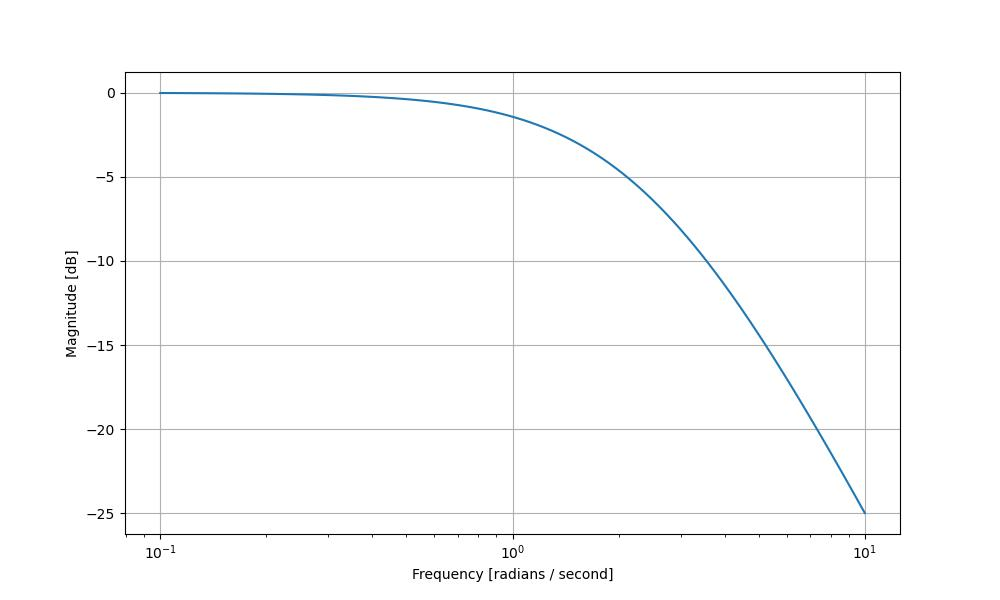
\includegraphics[width=\columnwidth]{2022/IN/15/figs/Figure_1.jpg}
\end{center}
\caption{Magnitude plot for the transfer function}
\end{figure}
\begin{figure}[!ht]
\centering
\begin{center}
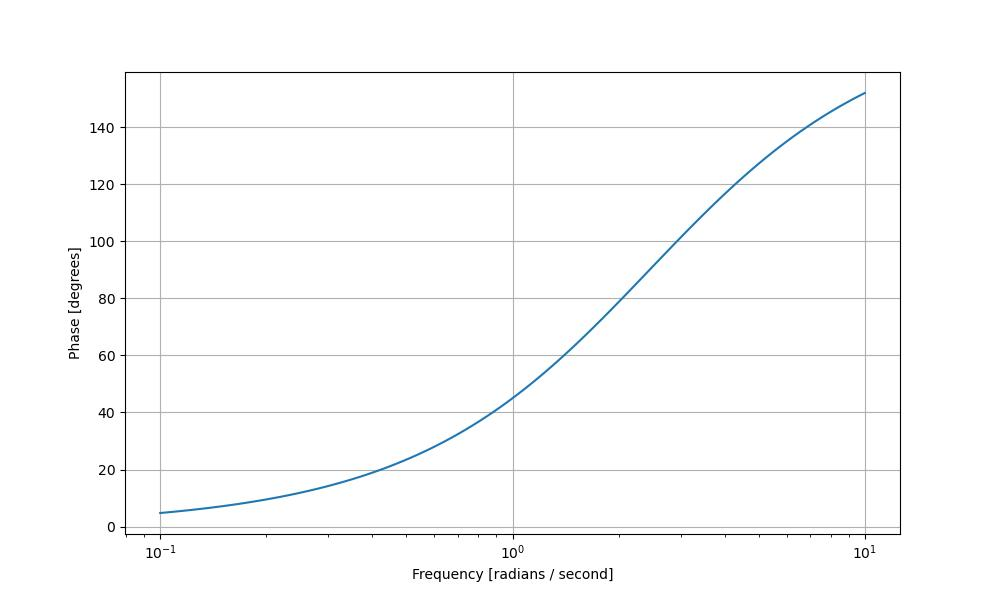
\includegraphics[width=\columnwidth]{2022/IN/15/figs/Figure_2.jpg}
\end{center}
\caption{Phase plot for the transfer function}
\end{figure}
